\documentclass{article}
\usepackage[utf8]{inputenc}
\usepackage{graphicx}
\usepackage{amsmath}
\usepackage{amssymb}

\title{\textbf{LINMA2471 : Optimization II - Models and Methods \\
Course Notes - 30th September 2015}}
\author{CHIEM Benjamin - 2174 1200\\
GERARD Céline - 2590 1200 \\
HAVELANGE Andine - 2583 1200 }
\date{October 2015}

\begin{document}

\maketitle

\subsection{Modelling Tricks}

After studying the standard form of some optimization problems, we will see some modelling tricks which permit to transform a non-linear or non-convex problem into a linear or convex optimization problem. 

\subsubsection{Monotonicity}

\newtheorem{mydef}{Definition}
\begin{mydef}
A monotonic function over an interval is a function that is either increasing or decreasing over this interval.
\end{mydef}

The transformation that is described in the following lines uses monotonic functions to turn an optimization problem into a simpler one. These operations do not change the problem but can change the solution and the optimal value of the objective of the problem. Let's see some examples. \\ 

\paragraph{Example 1}
$min \; \|x\|_{2}$ with $x \in X$ is equivalent to $min \; \|x\|_{2}^{2}$ with $x \in X$. In fact, $z \rightarrow z^2$ is a monotonic function (increasing in this case) over $\mathbb{R}$. By solving this problem, we will find the same optimal solution than the first model but the value of the objective function will be different. \\

\paragraph{Example 2}
These functions are monotonic and can be used like in the previous example to simplify the problem :
\begin{itemize}
\item[.]{$z \rightarrow e^z$}
\item[.]{$z \rightarrow log(z), \; (z>0)$}
\item[.]{$z \rightarrow -\frac{1}{z}, \; (z>0)$ for example, we can change $min \; \frac{1}{\|x\|_{2}}$ to $min \; -\|x\|_{2}$}\\
\end{itemize}

We not only use this trick to modify the objective function, but also some constraints. For example : 
$$f(x) \leq b \Leftrightarrow e^{f(x)} \leq e^{b}$$

\paragraph{Example  : Advertisement for bank account :}
This example allows us to look at the effects of monotonicity in real life optimization problems.
We put money into an account where we can't take our money back sooner than 5 years after. The bank guarantees that we have a high percentage when we take back our money after 5 years and assures the three rate over 3 years given on Figure \ref{ra}.\\ What is the worst global rate compatible with this ? Therefore, we are looking for the cumulative effect of the 5 rates (given over a year). 

\begin{figure}
\centering
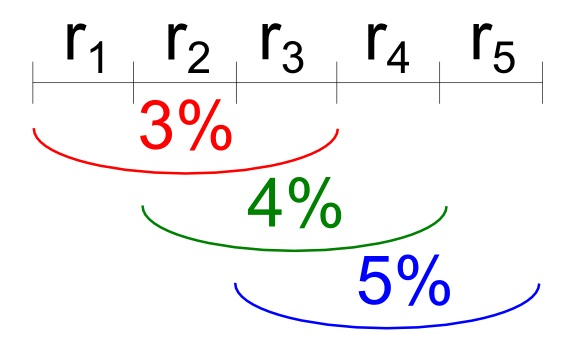
\includegraphics[scale=0.3]{rate.jpg}
\caption{Rates}
\label{ra}
\end{figure}

To solve this problem, we introduce the variables $r_i$ corresponding to the rate per year where $i = 1,...,5$. We don't want a rate which is negative or null so we have the following optimization problem :
$$\min \limits _{r_i > 0} r_1r_2r_3r_4r_5 $$
under the constraints : 
$$ r_1r_2r_3 \geq 1.03$$
$$ r_2r_3r_4 \geq 1.04$$
$$ r_3r_4r_5 \geq 1.05$$

This problem is not linear. We can transform it into a linear problem if we use the logarithm function. Indeed, let $y_i = log(r_i) \; \forall i=1,...,5$. We can do this because the logarithm is a monotonic increasing function. The problem can be written as : 
$$ min \; y_1 + y_2 + y_3 + y_4 + y_5$$
under the constraints : 
$$ y_1 + y_2 + y_3 \geq log(1.03)$$
$$ y_2 + y_3 + y_4 \geq log(1.04)$$
$$ y_3 + y_4 + y_5 \geq log(1.05)$$
This problem is now linear (and thus convex). \\

\textbf{Remark}\\
If we don't make the change of variable $y_i = log(r_i) \; \forall i=1,...,5$,  the variables $r_i$ appear in $log$ so the problem isn't linear.

\subsubsection{Change of variables}

We use change of variables in order to transform the problem into a linear or convex problem. For example, if every variable appears in a logarithm, then we can use the change of variable to remove the logarithm.\\ \underline{\textbf{NB}} : every appaerance of the variables needs to match the change of variables! \\

For example, signomials \footnote{A signomial is an algebraic function of one or more variables of the form:\\ $f(x_1,x_2,...x_n) = \sum_i{(c_i\prod_j{x_j^{a_{ij}}})}$} can be converted into convex functions thanks of this trick. Let's consider the signomial $\frac{x_1x_2^2}{x_3^{\frac{1}{2}}}$. Let $x_i = e^{y_i}$, we obtain the following expression by change of variable $e^{y_1+2y_2-\frac{1}{2}y_3}$. Moreover, the exponential of a linear function is convex and the change of variables conserves the convexity (See later).

\subsubsection{Misleading/Deceptive appearances}

In this part, we are looking for a polynomial $p(x), \; x \in \mathbb{R}$ of degree D which fulfils some characteristic (See Figure \ref{poly}): 
\begin{itemize}
\item[.]{For $x \in \left[0;f_1\right]$, $p(x) \geq 3$}
\item[.]{For $x \in \left[f_2;f_3\right]$, $p(x) \leq 0.5$} \\
\end{itemize}

Let $p(x) = \sum_{i=0}^{D} a_i x^{i}$.
On the Figure \ref{poly}, we observe that the polynomial will not be linear or convex. We then have the impression that the optimization problem is not linear. But it is not the case, given that the variables are not the $x_i$ but the $a_i$.
Furthermore, the constraints (2 examples of constraints are given below) are linear. 
$$ \sum_{i=0}^{D} a_i 50^{i} \geq 3 \Leftrightarrow p(50) \geq 3$$
$$ \sum_{i=0}^{D} a_i 100^{i} = 1 \Leftrightarrow p(100)=1$$

\begin{figure}[ht!]
\centering
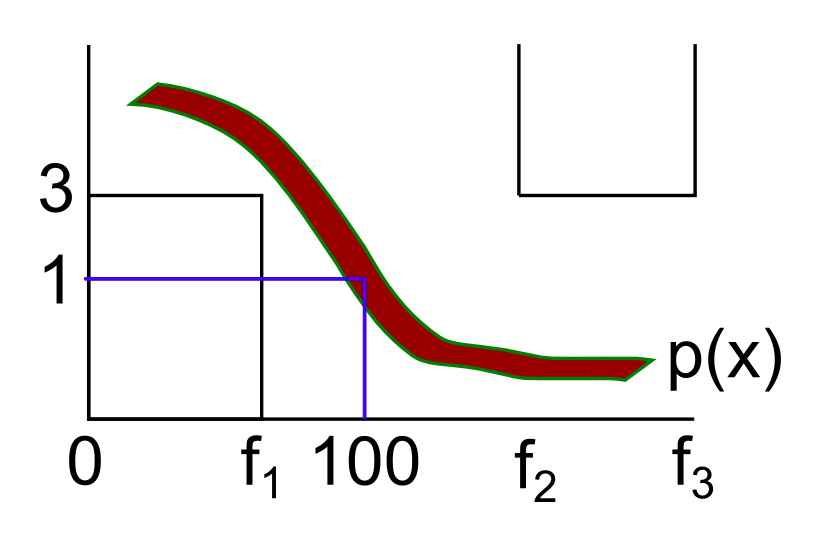
\includegraphics[scale=0.4]{poly.png}
\caption{Polynomial $p(x)$}
\label{poly}
\end{figure}

\subsubsection{Flexibility}
The flexibility of an optimization problem is its capacity to be solved in different ways depending on which criterion we really want to optimize. Let us consider an approximation problem. We have a set of points $(x_i,y_i)$ in $\mathbb{R}^2$, and we want to find the function (which is often a polynomial) which approximates \textit{at best} these points. In other words, we want to find a function $f$ that minimizes the errors $\epsilon _i$ at the approximation points:
\begin{eqnarray*}
\epsilon_i &=& |y_i - f(x_i)|
\end{eqnarray*}
The question now is to choose the way to minimize errors $\epsilon _i$. Indeed, we could choose to minimize overall errors with a least square criterion: 
\begin{eqnarray*}
\min ||\epsilon||_2 &=& \sqrt{\sum_i{\epsilon_i^2}}
\end{eqnarray*}
Another choice would be to minimize the sum of the errors:
\begin{eqnarray*}
\min ||\epsilon||_1 &=& \sum_i{|\epsilon_i|}
\end{eqnarray*}
Finally, a last (often used) way to minimize errors is to minimize the maximum error: 
\begin{eqnarray*}
\min\;\max_i \epsilon_i
\end{eqnarray*}
All these considerations prove that, depending on the criterion we choose to optimize (i.e. depending on the context), the result could be different. For example, the problem
\begin{eqnarray*}
\max &safety&\\
cost &\le& m
\end{eqnarray*}
will not lead to the same solution than
\begin{eqnarray*}
\min &cost&\\
safety &\ge& b
\end{eqnarray*}

\subsubsection{Charnes and Cooper}

Consider the non-linear problem which is a division of two linear expression : 
$$ \min \; \frac{c^{T}x + d}{f^{T}x + g}$$
under the constraints : 
$$ Ax \leq b$$

In this case, taking the logarithm of the objective function will not change anything: we will have the same problem. \\

We make the hypothesis that $f^{T}x+g > 0 \; \forall x \textit{ such that } Ax \leq b$. If not, we have the solution $-\infty$ which is not an interesting solution. \\

To solve this problem and make it linear, we are going to homogenize the objective function. Let $x = \frac{y}{t}$ with $y \in \mathbb{R}^{n}$ and $t >0 \in \mathbb{R}$. If we take $t=1$ then we get back to the original problem. So, one solution in $x$ correspond to several solutions in $(y,t)$ (for example : $(x,1), \; (2x,2), \; ... \; (\lambda x,\lambda)$).\\
We can write the problem as : 
$$ \min \; \frac{\frac{c^{T}y}{t}+d}{\frac{f^{T}y}{t}+g} $$
with : 
$$ A\frac{y}{t} \leq b$$

By simplification, we obtain the following problem : 
$$ \min \; \frac{c^{T}y + dt}{f^{T}y + gt}$$
with :
$$Ay \leq bt$$

Now, we notice that the objective function's numerator and denominator are linear as the constraint. This problem has a property called homogeneity. If you take any solution, you can multiply any component by the same constant and nothing changes. Mathematically : \\
$(y,t)$ solution $\Rightarrow (\lambda y, \lambda t)$ solution $\forall \lambda \ 0$ \\

We are gooing to choose solutions satisfying : $f^{T}y+gt=1$. We can do this using the property of homogeneity. This step results in selecting one solution among the collection of solutions multiple of each other. The objective function gets simpler and linear and we add one constraint. So, we have the following linear optimization problem : 
$$ \min c^{T}y + dt$$
with : 
$$ Ay-bt \leq 0$$
$$f^{T}y+gt = 1$$
$$t \geq 0$$

We compute $y^{*}$ and $t^{*}$ from this problem and take $x^{*} = \frac{y^{*}}{t^{*}}$ the solution of the original problem.\\ NOTE : If we have $t=0$ at the optimum then the problem is unbounded and $x^{*} \rightarrow \infty$. Example : 
$$ \min \; \frac{1}{x}$$
with : 
$$x \geq 1$$ 

This problem have an optimal value of 0 so the solution $x^{*} \rightarrow + \infty$. 

\subsection{Convex Optimization : Theorems and properties}
\subsubsection{Convex sets}
\underline{\textbf{Definition and examples}}

%\newtheorem{mydef}{Definition}
\begin{mydef}
A set X is convex if and only if
$$x,\;y \in X \Rightarrow \lambda x +(1-\lambda )y \in X \;\;\; \forall \; 0 \le \lambda \le 1$$
\end{mydef}

Thus, a set is convex if and only if it contains all the segments joining any pair of its points. \\

\textbf{Examples:}
\begin{itemize}
\item $\mathbb{R}^n$, $\mathbb{R}^n_+$, $\emptyset$
\item hyperplans ($\{x|\; b^Tx=\beta\}$)
\item open or closed half-spaces ($\{x|\;b^Tx<\beta\}$ and $\{x| \;b^Tx\le \beta\}$)
\item open and closed balls ($\{x|\;\|x-a\|<r\}$ and $\{x|\;\|x-a\|\leq r \}$)
\end{itemize}

\underline{\textbf{Properties}}
\newtheorem{myproperty}{Property}
\begin{myproperty}
Given a collection of convex sets $\{C_i\}_{i \in I} \subseteq \mathbb{R}^n$ ($I$ can be arbitrary), then $\bigcap \limits _{i \in I}C_i$ is convex too.
\end{myproperty}
It follows that polyhedrons are convex because they are intersection of half-spaces.\\

%\newtheorem{myproperty}{Property}
\begin{myproperty}
Given a collection of convex sets $C_1,\; C_2,\; C_3,\; ....\;C_n$, their cartesian product $C_1\times C_2 \times C_3 \times ... \times C_n$ is convex too. 
\end{myproperty}

%\newtheorem{myproperty}{Property}
\begin{myproperty}
If $X\subseteq \mathbb{R}^n$ and $X\subseteq \mathbb{R}^n$ are convex then the Minkowski sum of $X$ and $Y$, $X+Y=\{x+y\;|\;x \in X \;\text{and} \; y \in Y\}$ is convex too. 
\end{myproperty}

\textbf{Remark}\\
The union of convex sets is not always convex! 
\\

\subsubsection{Convex functions}
\underline{\textbf{Definition and examples}}
%\newtheorem{mydef}{Definition}
\begin{mydef}
A function f with domain D is a convex function of and only if \\
\begin{center}
D is convex and 
\end{center}
$$x,y\; \in D \Rightarrow f(\lambda x+(1-\lambda)y) \le \lambda f(x)+(1-\lambda)f(y) \;\;\; \forall \; 0\le \lambda \le 1$$
\end{mydef}

\textbf{Examples:}
\begin{itemize}
\item linear and affine functions are convex ($x \rightarrow \alpha x$,  $x\rightarrow b^Tx$  and  $x \rightarrow b^Tx+\alpha$)
\item the norm function and the square of the norm function are convex functions ($x \rightarrow \|x\|$ and $x \rightarrow \|x\|^2$)
\item quadratic forms ($x \rightarrow x^TQx$) are convex functions when the matrix $Q \in \mathbb{R}^{n\times n}$ is semi positive definite
\item the functions $x \rightarrow e^x$,  $x\rightarrow log(x)$ and $x \rightarrow |x|^p \;\;(1 \le p)$ are convex
\end{itemize}


%\newtheorem{mydef}{Definition}
\begin{mydef}
A function $f$ is concave $\Leftrightarrow$ $-f$ is convex.
\end{mydef}

\textbf{Remark}\\
Linear and affine functions are convex and concave. 
\\
\\

\underline{\textbf{Properties}}\\

To know whether a function is convex or not, we have to transform it into its epigraph and check if it is convex or not. But there are some useful properties of convex functions that we can use to spare time. 

%\newtheorem{myproperty}{Property}
\begin{myproperty}
If $f$ is a convex function and $c \in \mathbb{R}_0^+$, then $cf$ is convex.  
\end{myproperty}

%\newtheorem{myproperty}{Property}
\begin{myproperty}
If $f$ and $g$ are convex functions, then $f+g$ is convex. 
\end{myproperty}

%\newtheorem{myproperty}{Property}
\begin{myproperty}
Given a collection of convex functions $\{f_i\}_{i \in I}: \mathbb{R}^n \rightarrow \mathbb{R}$, \\
$\sup \limits _{i \in I}f_i$ is convex too. 
\end{myproperty}
with $\left[ \sup \limits _{i \in I} f_i\right] (x)= \sup \limits _{i \in I} f_i(x)$

%\newtheorem{myproperty}{Property}
\begin{myproperty}
Given $f(x,s)$ (with $x \in \mathbb{R}^n$ and $s \in \mathbb{R}$, a parameter) such that $x \rightarrow f(x,s)$ is convex for any $s$, 
$$\int_{s \in S}f(x,s)ds\;\; \text{is \;convex}$$
\end{myproperty}

\bigskip

\bigskip

\underline{\textbf{Convexity and differential calculus}}
%\newtheorem{myproperty}{Property}
\begin{myproperty}
Let $f$ be a differentiable function of which the domain D is open. 
$f$ is convex if and only if D is convex and
$$\forall x,y \; \in D, \;f(y)\geq f(x)+\nabla f(x)^T(y-x) $$
\end{myproperty}
This property means that, if $f$ is convex, it will be above all its Taylor approximations of first order. This signifies that at any point, the tangent of the function is under the function. This is useful to make a piecewise approximation of $f$ by linear functions (an example of such an approximation is shown on Figure \ref{ApproximationConvexe}). In order to obtain such an approximation, we have to choose $n$ points at which we calculate the tangent of the function $f$ and then take the maximum of the $n$ tangents (in the example, $n=3$). \\
Besides, the value of the approximation is lower than the real value on any point. It allows us to obtain lower bounds. 
\\

\begin{figure}[ht!]
\centering
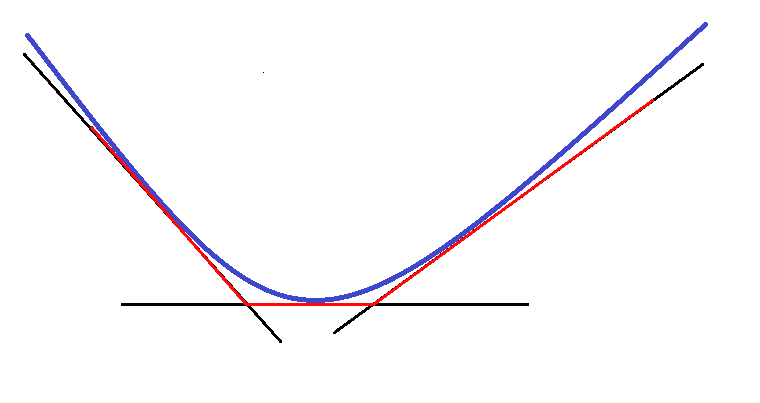
\includegraphics[scale=0.4]{ApproximationConvexe.png}
\caption{Illustration of the piecewise linear approximation of a convex function}
\label{ApproximationConvexe}
\end{figure}

%\newtheorem{myproperty}{Property}
\begin{myproperty}
Let $f$ be a twice differentiable function of which the domain D is open. 
$f$ is convex if and only if D is convex and
$$\forall x\in D,\; \nabla^2f(x)\geq 0 $$
\end{myproperty}

\subsubsection{Convexity and linear transformations}
Linear transformations preserve convexity. Indeed,

%\newtheorem{myproperty}{Property}
\begin{myproperty}
If $S\subseteq \mathbb{R}^n$ is convex and $\Phi: \; \mathbb{R}^n \rightarrow \mathbb{R}^m: \; x \rightarrow Ax+b$ is a linear transformation, then
the image of $S$ by $\Phi$,
$$\Phi (S)=\{\Phi(x)|\; x \in S\}$$
is convex too. 
\end{myproperty}

%\newtheorem{myproperty}{Property}
\begin{myproperty}
If $\Phi: \; \mathbb{R}^n \rightarrow \mathbb{R}^m: \; x \rightarrow Ax+b$ is a linear transformation and $f:x\rightarrow f(x)$ is a convex function, then
the composition 
$$f\circ \Phi=f(\Phi(x))=f(Ax+b)$$
is convex too. 
\end{myproperty}

%\newtheorem{myproperty}{Property}
\begin{myproperty}
If $S\subseteq \mathbb{R}^n$ is convex and $\Theta: \; \mathbb{R}^m \rightarrow \mathbb{R}^n: \; x \rightarrow ax+b$ is a linear transformation, then
the image of $S$ by the inverse of $\Theta$,
$$\Theta ^{-1} (S)=\{x|\;\Theta (x) \in S\}$$
is convex too. 
\end{myproperty}













\end{document}
